\chapter{Fernsteuerungsschnittstelle}
\chapterauthor{Matthias Greil}
Die Steuerung von Smart Drive ist über eine UART-Schnittstelle vorgesehen. Die
ermöglicht alle Typischen RC-Controller Schnittstellen, wie S-Bus, I-Bus, CRSF
wie auch weiter oder Eigene Lösungen zu verwenden. Da bei den Test der
\textit{T8L-Radio-Controller (M2)} \cite{t8l_controller} und der \textit{XR1 Nano Multi-Frequency ExpressLRS
Receiver} \cite{XR1_reciver} von Radiomaster genutzt wurden, wurde das CRSF-Protokoll implementiert. Jegliche anderen Protokolle wurden nicht implementiert. 

%TODO: Blockschaltbild wie steuerung aufgebaut ist: vernsteuerung ))) reciver ->
%CRSF an UART Port am MCU

 \section{Verwendeter RC-Fernsteuerung}
 Die Verwendete RC-Fernsteuerung ist die \textit{T8L Radio Controller (M2)}
 \cite{t8l_controller} von Radiomaster. Sie wurde gewählt, da sie im Vergleich
 mit Fernsteuerungen mit den gleichen Features, am günstigsten ist. Sie
 supported das ExpressLRS Protokoll auf 2.4GHz. Als Empfänger wurde ein
 \textit{XR1 Nano Multi-Frequency ExpressLRS Receiver} \cite{XR1_reciver} von
 Radiomaster genutzt. Diese unterstützt auch das ExpressLRS Protokoll auf
 2.4GHz. Die empfangen Daten werden über das das CRSF Protokoll der
 Steuerplatine übertragen.

\noindent
\begin{minipage}[c]{0.5\textwidth}
    \centering
    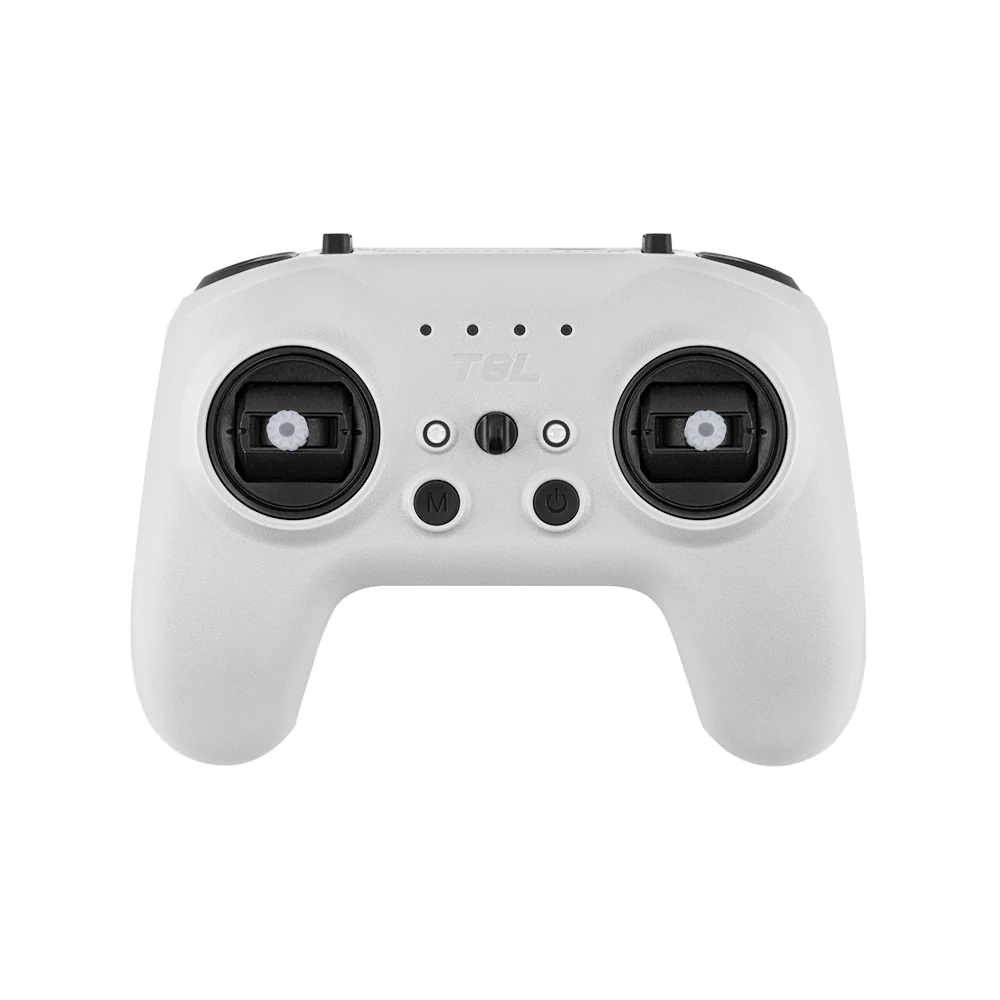
\includegraphics[width=\linewidth]{Bilder-Grafiken/Matthias/Fernsteuerung/T8L-RC-Controller.png}
    \captionof{figure}{Radiomaster T8L (M2) \cite{t8l_controller}}
\end{minipage}
\hfill
\begin{minipage}[c]{0.4\textwidth}
    \centering
    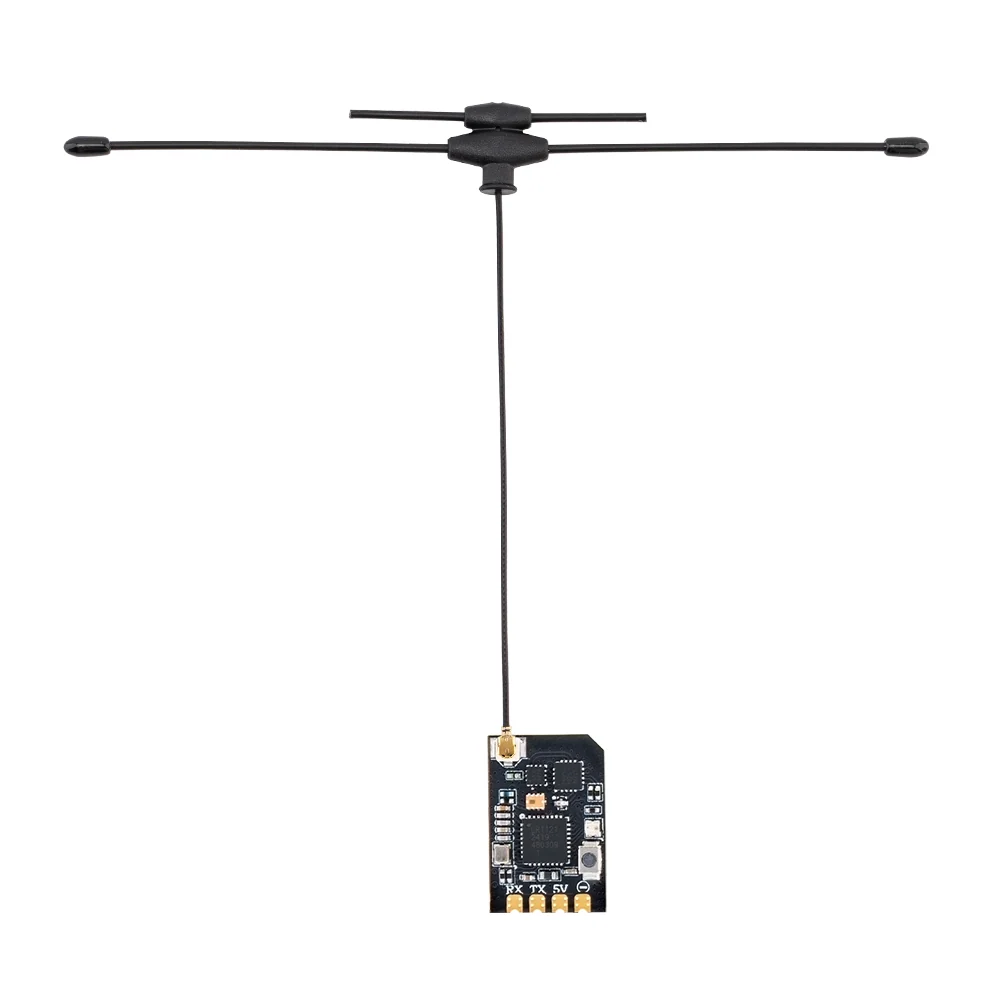
\includegraphics[width=\linewidth]{Bilder-Grafiken/Matthias/Fernsteuerung/XR1_Reciver_Bild.png}
    \captionof{figure}{Radiomaster XR1 Nano Multi-Frequency ExpressLRS Receiver
    \cite{XR1_reciver}}
\end{minipage}
\newpage
  


\section{CRSF-Protokoll}
CRSF ist ein Protokoll \cite{crsf_protokoll_spec} das für die Kommunikation von Radio Controlled (RC)
Geräten genutzt wird. Anders als wie bei z.B. S-Bus sind die Frame-Größen nicht
konstant, sondern werden auf Größe des Pakets angepasst. Das machte es zu einem
sehr flexiblen Protokoll, dass unter anderem die RC-Kanäle der Fernsteuerung, GPS
Daten und Übertragungsqualität übertragen kann, wie auch vieles weiteres.

\subsection{Aufbau eines Frames}
Der Anfang eines Frames ist immer gleich Aufgebaut. Es gibt einen Start Byte
(0xC8), Frame Länge und der Frame-Type. Danach folgt die Payload, die unterschiedlich lang
sein kann. Am Ende des Frames sitzt immer der CRC. Frames müssen mindestens 4
Byte lang sein und maximal 64 Byte.
\begin{figure}[h]
    \centering
    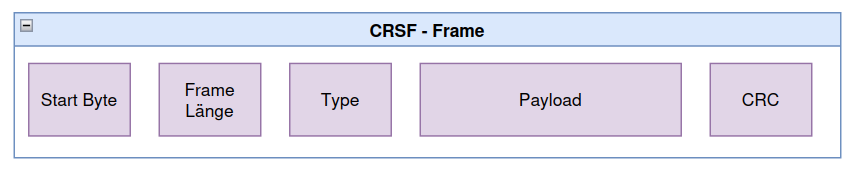
\includegraphics[width=\textwidth]{Bilder-Grafiken/Matthias/Fernsteuerung/CRSF-Frame.png}
    \caption{Aufbau des CRSF-Frames \cite{crsf_protokoll_spec}}
\end{figure}

\subsection{Protokoll Schnittstelle}
Das CRSF-Protokoll wird wie die meisten anderne RC-Fernsteuerungsprtokolle über
UART übertragen. In der CRSF-Specification \cite{crsf_protokoll_spec} werden
drei Arten der Schnittstellen beschrieben. \grqq Single-Wire Half-Duplex
UART\grqq, \grqq Dual-Wire Full-Duplex UART\grqq und \grqq Multi-master I2C
(BST)\grqq. Die Schnittstelle die der Radiomasterr XR1 Nano supported ist die
Full-Duplex UART schnittstelle.\\
Laut Specification ist diese defaultmäßig auf eine 416666 Baudrate, 8N1 (8 Daten
Bits, keine Parität, und in Stopp-Bit) eingestellt. Sie muss mit 3.0 - 3.3 Volt
betrieben werden. Das UART Signal ist nicht invertiert, anders wie bei anderen
RC-Protokollen (z.B. S-Bus).


\section{Architektur der CRSF-Protokollverarbeitung} 
Es wurde sich die Architektur und Implementation der CRSF-Protokollverarbeitung
bei Betaflight und Ardupilot analysiert. Betaflight ist \grqq die Weltweit
führende Multi-Rotor Flight-Controller Software\grqq.
Ardupilot ist ein Autopilot System das unterschiedliche arten
von Fahrzeugen supported. Beide sind Open Source. Es wurde sich damit befasst
wie diese zwei Projekte die Kommunikation mit dem RC-Receiver implementieren.

\newpage
\subsection{Betaflight}
Das Empfangen vom CRSF-Protokoll ist bei Betaflight Interrupt basiert
\cite{betaflight_crsf}.
Bei einem neu Empfangen Byte, löste der Rx-Interrupt aus. In diesem wird der
Byte in ein Statisches Array kopiert. Auch das Parsen wird direkt im 
Interrupt durchgeführt. In Abbildung
\ref{fig:flussdiagramm_betaflight} wird ein vereinfachter Ablauf 
der Interrupt Routine gezeigt. Wenn ein ganzes Frame Empfangen ist, wird
dieser im Scheduler weiter verarbeitet.

\begin{figure}[h]
    \centering
    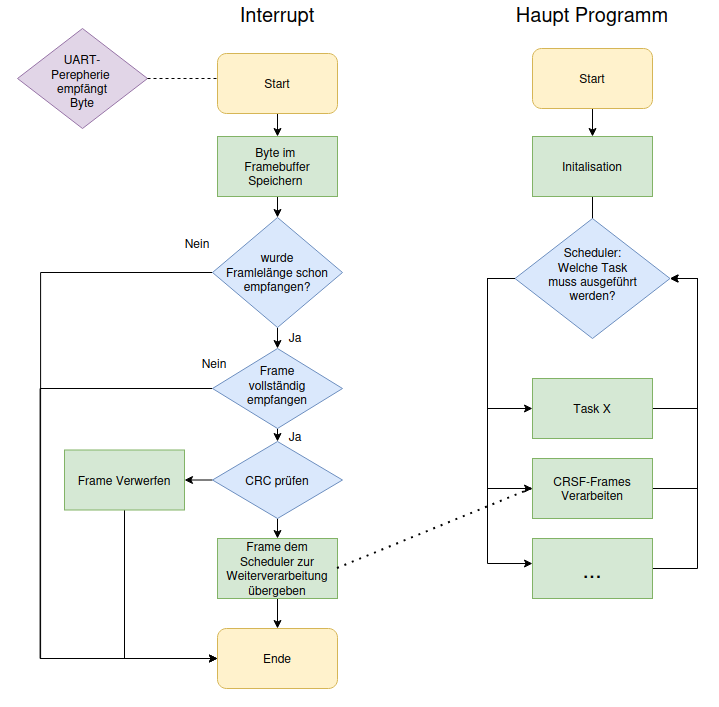
\includegraphics[width=0.95\textwidth]{Bilder-Grafiken/Matthias/Fernsteuerung/CRSF-Betaflight-Software.png}
    \caption{Betaflight - Empfang und Verarbeitung von CRSF-Frames}
    \label{fig:flussdiagramm_betaflight}
\end{figure}

\noindent
Erwähnenswert ist bei Betaflighs sehr viel des Empfangensprozess im Interrupt
verarbeitet. Die ISR im Sourcecode ist fast 150 Zeilen lang. Natürlich ist die
Zeilenanzahl ungleich der Ausführungszeit, veranschaulicht aber das sehr viel in
diesem Interrupt passiert. Das ist insoweit problematisch, da während des
Interrupts, der Prozessor auf nichts weiteres reagieren kann.

% --- BEGINN Ardupilot-Teil (von Claude eingefügt) ---
\newpage
\subsection{Ardupilot}
Anders als bei Betaflight nutzt Ardupilot eine DMA-Einheit
um den CRSF-Frame zu empfangen \cite{ardupilot_crsf}. Erst wenn ein
vollständiger Frame empfangen ist, wird ein sogenannter IDEL-Line-Interrupt
ausgelöst, mit diesem Interrupt wird die Verarbeitung gestartet.
Es ist zu erwähnen das Ardupilot ein Real time Operation System (RTOS) namens
ChibiOS nutzt. Die Verarbeitung der empfangenen Daten passiert in einer
Thread. In Abbildung
\ref{fig:flussdiagramm_ardupilot} wird ein vereinfachter Ablauf 
des Programmcodes gezeigt.

\begin{figure}[h]
    \centering
    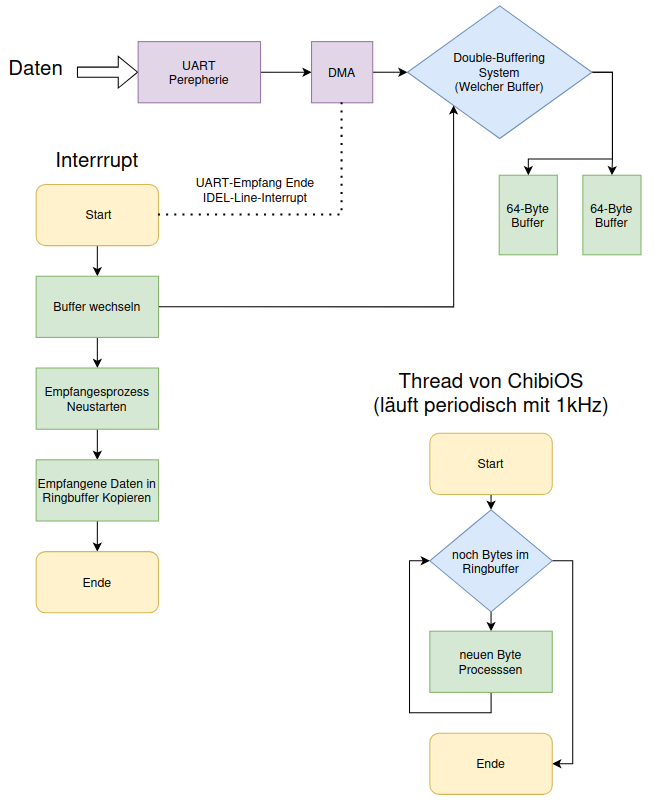
\includegraphics[width=0.75\textwidth]{Bilder-Grafiken/Matthias/Fernsteuerung/CRSF-Ardupilot-Software.png}
    \caption{Ardupilot - Empfang und Verarbeitung von CRSF-Frames}
    \label{fig:flussdiagramm_ardupilot}
\end{figure}

Da für den Empfang eine DMA-Einheit genugzt wird, wird die CPU gebraucht,
außer am Frame-Ende. Der ausgelöste Interrupt, wechselt den Buffer, in den
die DMA-Einheit schreibt, startet die Empfangensprozess neu und schreibt die
empfangenden Daten in einen seperaten Ringbuffer. Dieser Ringbuffer wird über
eine Thread in einem 1kHz Takt ausgelesen. Dadurch werden keine
Interrupts durch das Verarbeiten blockiert.

\subsection{Vergleich der Ansätze von Betaflight und Ardupilot}
Betaflight und Ardupilot nutzen verschiedene Ansätze zur Empfangung des
Protkolls. Betaflight verfolgt einen simplere Architektur, in der
alles über Interrupts verarbeitet wird. Erst wenn bestätigt ist, dass
sein Frame richtig empfangen wurde, wird die in dann durch eine Task in
einem Scheduler fertig verarbeitet. Ardupilot offloaded das Empfangen an rein
an die Hardware und nur einen kurzen Interrupt um den Empfangensprozess neu
zu starten. Das Verarbeiten wird rein in einer Thread
durchgeführt.\\
Ardupilot erzeugt somit weniger und dann kürzere Interrupts,
(zeit-)kritischere Interrupts blockieren könnte. Wobei es mit mehr Komplexität in der Implementierung folgt. 

\section{Gewählte Architektur für SmartDrive X4}
Bei der Implementierung wurde sich stark an Ardupilot orientiert. Es gibt aber
statt dem Doulbe-Buffering-System + Ringbuffer einen einzigen 512Byte großen 
Ring-Buffer, der direkt von der DMA-Einheit beschieben wird. Es werden nur bei Fehlern Interrupts
ausgelöst, der Rest wird im Hauptprogramm mit 100Hz verarbeitet. Pro Periode
werden alle neuen Daten geparsed, somit wird der aktuellste Frame jedes
Frametypen gespeichert. Dadurch das
alle Empfangen Daten im Buffer landen, ist das verarbeiten nicht Zeitkritisch.\\

Der Frame-Parser iteriert beim Start durch den Rinbbuffer bis er die Adresse für
Flight Contorller gefunden wird. Diese ist der Start des Frames. Alle Frame-Bytes
werden in einem Zwischen-Buffer gespeichert. Sobald das Ende des Frames erreicht
wurde, muss die Korrekte Übertragung mit der CRC-Checksumme überprüft werden.
Erst danach Kann der Frame-Inhalt verarbeitet werden. Dies muss für jeden
Fragetyp individuell getan werden. 

\begin{figure}[H]
    \centering
    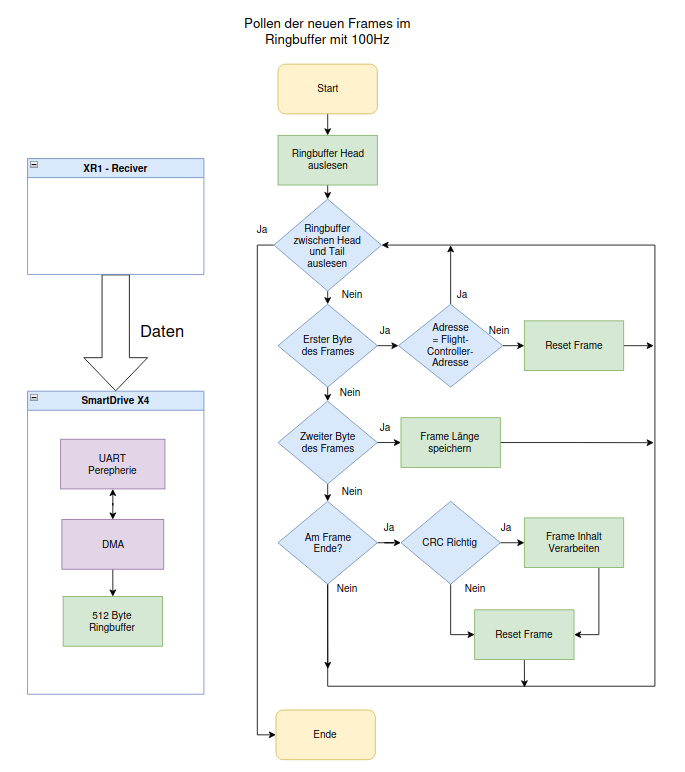
\includegraphics[width=1\textwidth]{Bilder-Grafiken/Matthias/Fernsteuerung/CRSF-SmartDriveX4-Software.png}
    \caption{Eigenimplementierung - Empfang und Verarbeitung von CRSF-Frames}
    \label{fig:flussdiagramm_smartdrivex4}
\end{figure}

\newpage

\subsubsection{Ring Buffer Dimensionierung}
Ein Problem dieses Buffers ist, dasss der Ringbuffer überlaufen kann.
Besonders wenn der Prozessor gerade andere rechenintensiven Teile des Programms
verarbeitet und dort aufgehalten wird. Daher muss der Buffer groß genug
gewählt werden, so dass genug reserve existiert um Verzögerungen in
der Verarbeitung ausgleichen zu können. Ein zu großer Buffer verschwendet
jedoch RAM.\\ 
Die Radiomaster T8L (M2) \cite{t8l_controller} und das CRSF-Protokoll unterstützt mehrere Update
Raten von 100Hz bis zu 1kHz. Diese sind am T8L einstellbar. Es muss der buffer für die Maximale Update
Frequenz und Frame-Größe dimensioniert werden. Es wurde folgende Formel
genutzt um die Zeit zu bestimmen, bis der Buffer überfüllt ist. Wobei:\\
$N_{Buf}$ ... Ringbuffer-Größe in Bytes\\
$n_{max}$ ... Maximale Frame-Größe in Bytes\\
$f$ ... Updaterate in Hz

\[
    T_{overflow} =\frac{N_{Buf}}{n_{max}} \cdot \frac{1}{f}
\] 

\[
    \frac{512 \text{Bytes}}{64 \text{Bytes}} \cdot \frac{1}{100 \text{Hz}} = 80ms
\] 
\[
    \frac{512 \text{Bytes}}{64 \text{Bytes}} \cdot \frac{1}{250 \text{Hz}} = 32ms
\] 
\[
    \frac{512 \text{Bytes}}{64 \text{Bytes}} \cdot \frac{1}{500 \text{Hz}} = 16ms
\] 
\[
    \frac{512 \text{Bytes}}{64 \text{Bytes}} \cdot \frac{1}{1 \text{kHz}} = 8ms
\] 
Aus diesen Rechnungen geht hervor, dass die Buffer-Größe bei 100Hz und 250Hz
ausreichend ist, wenn alle 10ms gepolled wird. Noch dazu muss eine gewisse Verzögerung
eingeplant werden, sie wurde mit unter 10ms angenommen. 
Ab 500Hz ist die $\text{Pollingzeit} + \text{Verzögerung}$ sehr knapp vor einem
Überlauf. Ab 1kHz ist die Buffer-Größe zu klein.\\
Es wurde trotzdem 512Bytes als Buffer-Größe gewählt, da in Theorie das
CRSF-Protokoll Übertragungsgeschwindigkeiten bis zu 1kHz supported. Dies kann am
Contorller eingestellt werden. Mehr als 250Hz wird in Praxis nicht gebraucht.\\
Die gewählte Formel beschreibt nur die Maximalauslastung. In Betrieb sind
die meisten Frames unter 64Bytes lang. Somit ist die Auslastung des Ringbuffers
geringer als berechnet.

